\documentclass[tikz,border=2pt]{standalone}
\usepackage{amsmath}
\usepackage{pgfplots}
\pgfplotsset{compat=1.18}
\usepgfplotslibrary{fillbetween}
\usetikzlibrary{calc}

\begin{document}
% Left: the area under f on [a,b]. Right: an antiderivative F; the area equals the rise F(b)-F(a).
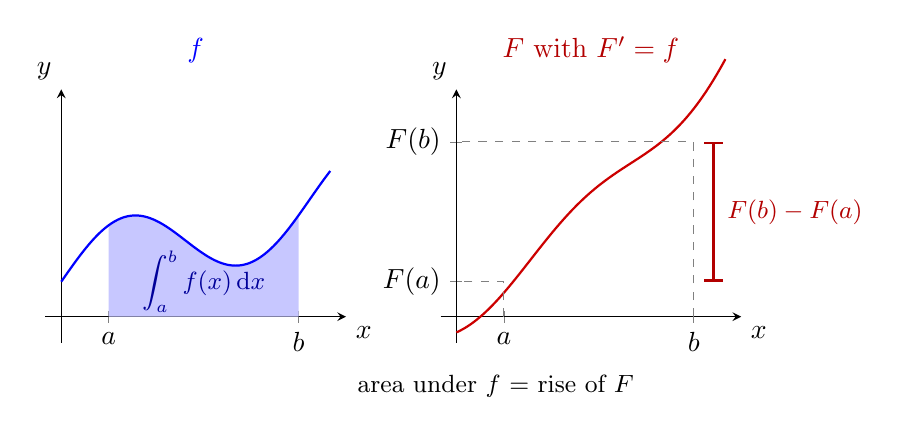
\begin{tikzpicture}
	\begin{axis}[
		name=left,
		axis lines=middle,
		xmin=-0.2, xmax=3.6,
		ymin=-0.3, ymax=2.6,
		xtick={0.6,3.0}, xticklabels={$a$,$b$},
		ytick=\empty,
		xlabel={$x$}, ylabel={$y$},
		xlabel style={below right}, ylabel style={above left},
		samples=120, smooth, clip=false,
		width=5.4cm, height=4.8cm,
		title={$f$}, title style={blue}
		]
		\addplot[name path=f, thick, blue, domain=0:3.4] {0.4+0.3*x+0.5*sin(deg(2*x))};
		\addplot[name path=ax, draw=none, domain=0:3.4] {0};
		\addplot[blue!22] fill between[of=f and ax, soft clip={domain=0.6:3.0}];
		\node[blue!60!black, font=\small] at (axis cs:1.8,0.4) {$\displaystyle\int_a^b f(x)\,\mathrm{d}x$};
	\end{axis}
	\begin{axis}[
		at={(left.east)}, anchor=west, xshift=1.2cm,
		axis lines=middle,
		xmin=-0.2, xmax=3.6,
		ymin=-0.3, ymax=2.6,
		xtick={0.6,3.0}, xticklabels={$a$,$b$},
		ytick={0.4,2.0}, yticklabels={$F(a)$,$F(b)$},
		xlabel={$x$}, ylabel={$y$},
		xlabel style={below right}, ylabel style={above left},
		samples=120, smooth, clip=false,
		width=5.4cm, height=4.8cm,
		title={$F$ with $F'=f$}, title style={red!70!black}
		]
		% F(x) = 0.4x + 0.15x^2 - 0.25 cos(2x) + 0.25 ; F(0.6)≈0.40, F(3.0)≈2.0 (rescaled sketch)
		\addplot[thick, red!80!black, domain=0:3.4] {0.4*x+0.15*x^2-0.25*cos(deg(2*x))+0.07};
		\draw[dashed, gray] (axis cs:0.6,0) -- (axis cs:0.6,0.4) -- (axis cs:0,0.4);
		\draw[dashed, gray] (axis cs:3.0,0) -- (axis cs:3.0,2.0) -- (axis cs:0,2.0);
		\draw[red!70!black, thick, |-|] (axis cs:3.25,0.4) -- (axis cs:3.25,2.0);
		\node[red!70!black, anchor=west, font=\small] at (axis cs:3.3,1.2) {$F(b)-F(a)$};
	\end{axis}
	\node[font=\small] at ($(left.south east)+(1.9,-0.55)$) {area under $f$ $=$ rise of $F$};
\end{tikzpicture}
\end{document}
